\subsection{Motivation von Sensornetzen}\label{ss:MotivationSensornetze}

Sensornetze sind sehr flexibel und können unter anderem dafür eingesetzt werden, um
\begin{itemize}
	\item Umwelteinflüsse wahrzunehmen ('sensing')
	\item Umwelteinflüsse zu verarbeiten und zu analysieren ('computing')
	\item Daten zu übertragen ('transport')
	\item Netzwerke für verteile Systeme aufzubauen ('networking')
	\item Die Umwelt zu beeinflussen und zu verändern ('actuation')
\end{itemize}

F\"ur viele Anwendungsfälle und Szenarien, in denen mit der Umwelt interagiert wird, soll die Benutzung von drahtlosen Sensornetzen zukünftig ausgebaut und etabliert werden. Der Einsatz von Sensornetzen kann dabei verschiedene Motivationen und Anforderungen haben:
\begin{itemize}
	\item Direkte Interaktion mit Menschen ist nicht möglich oder nicht erforderlich (z.B. bei Überwachung einer Maschine in der Industrie)
	\item Der Mensch soll nur im Notfall alarmiert werden (z.B. in Notfällen oder wenn die Sensoren bestimmte Schwellenwerte erreichen)
	\item Es handelt sich um ein autonomes System, welches nur Selten das Handeln eines Menschen erfordert
\end{itemize}

\begin{figure}[H] 
	\centering
	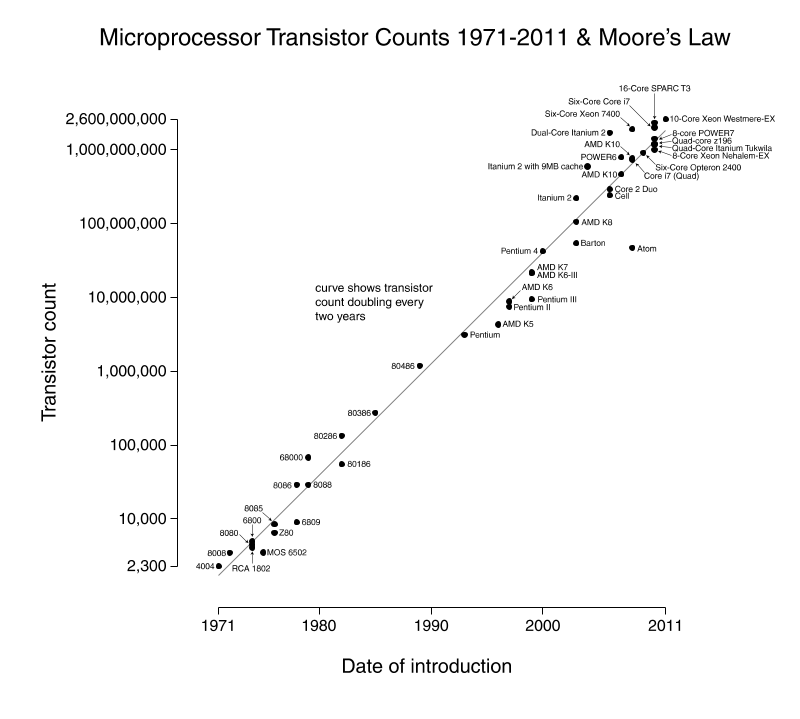
\includegraphics[scale=0.5]{Bilder/mooreslaw}
	\caption{Mikroprozessoren-Transistoren im Laufe der Zeit\cite{i:mooreslaw}}
	\label{f:mooreslaw}
\end{figure}

Eine weitere Motivation der Verwirklichung von drahtlosen Sensornetzen ist der Technologiefortschritt, der es möglich macht, immer kleinere Rechengeräte mit mehr Leistung herzustellen und miteinander zu vernetzen. Um diesen Fortschritt zu verdeutlichen, formulierte Gordon Moore 1965 ein Gesetz, welches besagt, dass sich die Anzahl der integrierten Schaltkreise auf einem Mikroprozessor alle 18-24 Monate verdoppelt. Im Gegensatz zu den Anzahl der Schaltkreise steigt die Rechenleistung der Prozessoren allerdings nicht linear an, da immer mehr Schaltkreise für den Cache des Prozessors verwendet werden, was nur geringfügig der Leistungssteigerung dient. Das Ende der Gültigkeit des Mooreschen Gesetzes wurde schon des öfteren wegen unüberwindbarer technischer Grenzen vorausgesagt, diese wurden jedoch bisher alle mit dem Einsatz neuer technischen Mittel und Materialien überwunden. Momentan schätzt der Halbleiterhersteller Intel, welcher 1968 von Moore mitbegründet wurde, dass das Mooresche Gesetz noch mindestens bis 2023 seine Gültigkeit behält. Mittlerweile existieren beim Konzern sogar explizite Pläne, die das Einhalten des Mooreschen Gesetzes sicherstellen sollen.  \cite{d:wolf} \cite{d:kahle} \cite{d:tuomi}. \\
